\tocless\subsection{Desciption du jeu}
Film iconique des années 1980, \textbf{Tron} est une science-fiction américain réalisé par
Steven Lisberger au sein de l'entreprise Walt Disney Pictures. Ce dernier met en scène un jeu dans 
un monde virtuel où des motos futuristes se déplacent à une vitesse constante, n'effectuant que des 
virages à angle droit\footnote{Les virages à angle droit sont des virages où la nouvelle direction 
est perpendiculaire à la direction précédente.} 
\begin{figure}[h!]
	\centering
	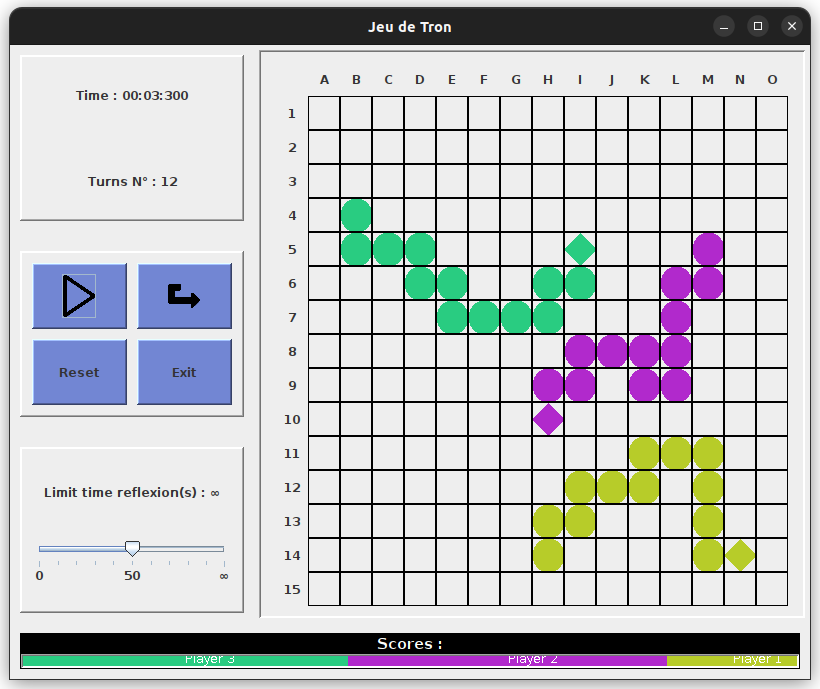
\includegraphics[scale=0.35]{Images/jeu-tron.png}
	\caption{Jeu de Tron}
	\label{fig:jeu-tron}
\end{figure}
et laissant derrière elles des trainées solides. Ainsi,
au fur et à mesure que le jeu avance, le plateau se remplit de murs et finalement un ou plusieurs
joueurs se retrouvent coincés dans un cul-de-sac. Le but du jeu est de survivre le plus longtemps et 
d'être le dernier survivant. Ce jeu est devenu très populaire et a ensuite été implémenté sur diverses
plateformes et diverses versions.\\
\tocless\subsection{Analyse mathématiques du jeu}
\textbf{Tron} est un jeu se jouant sur une grille de taille $N\times M$ avec $N$ et $M$ entiers positifs. Chaque 
cellule de la grille peut être \texttt{vide} ou \texttt{occupée} par un joueur. Généralement, la grille 
considérée est carrée, c'est à dire $N=M$. C'est un jeu multijoueur dans lequel les $K$ joueurs, à 
chaque tour, font un choix:
\begin{itemize}
	\item \texttt{continuer} dans la même direction
	\item \texttt{tourner} à $90^{\circ}$ à gauche ou à droite
\end{itemize}
Un joueur ne peut pas s'arreter et doit toujours se déplacer. C'est un jeu assez rapide, car les
joueurs se déplacent à une vitesse constante($\approx 100ms$ par tour). Tous les choix sont fait 
de manière simultanée ce qui rend le jeu très dynamique et complexifie l'anticipation des mouvements
des adversaires. Le jeu se finit avec 2 états possibles:
\begin{itemize}
	\item \texttt{victoire} d'un joueur, si il est le dernier survivant
	\item \texttt{nulle} si tous les joueurs sont éliminés
\end{itemize}

Plus en détail, à chaque sequence discrète de temps $t=0,1,2,...$, les joueurs $i=1,2,...,K$ reçoivent 
une même représentaion $s_t \in S$ de l'état du jeu, où $S$ est l'espace des états possibles. 
%Integrer un fichier
\begin{figure}
	\centering
	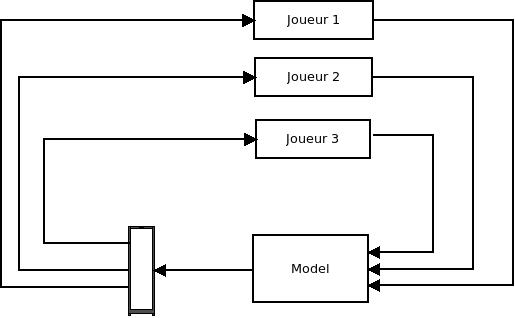
\includegraphics[scale=0.4]{Images/interraction_model.jpeg}
	\caption{Modèle d'interraction entre 3 joueurs}
	\label{fig:modele-interraction}
\end{figure}
En fonction de l'état $s_t$, chaque joueur $i$ choisit une action $a_{i,t} \in A_i(s_t)$, où $A_i(s_t)$
est l'espace des actions possibles pour le joueur $i$ dans l'état $s_t$. Ainsi, chaque joueur $i$. Comme conséquence,
chaque joueur $i$ reçoit une nouvelle représentation $s_{t+1} \in S$ de l'état courant du jeu.\ref{fig:modele-interraction}


Ainsi le jeu de Tron est un jeu ayant une longueur fini. En effet, le nombre d'étape nécessaire 
pour terminer le jeu est majoré par :
\begin{equation}
	\label{eq:nb-etapes}
	\frac{N\times M}{K}
\end{equation}
où $N$(resp. $M$) est la taille de la grille en largeur (resp. en hauteur) et $K$ est le nombre de joueurs.\\
Toutefois en pratique, le jeu peut se terminer plus ou moins rapidement en fonction de la stratégie
des joueurs.